\section{Set up}
{GRASP Builder application can be executed in both operating systems, Windows and Linux.
The only prerequisite in order to work with this application is to have MATLAB installed.
\smallskip\\The only functionality not enabled in Windows is the execution of GRASP algorithm, since this application is designed to work in CALCULA environment, but all the other functionalities can be used, if the user prefers.}
\subsection{Windows}
{Since this application is not being installed with any executable or saved in registry, it is only necessary to unzip file \textit{GRASP\_Builder\_Release\_Windows.zip} in the desired folder.}
\begin{figure}[H]
\centering
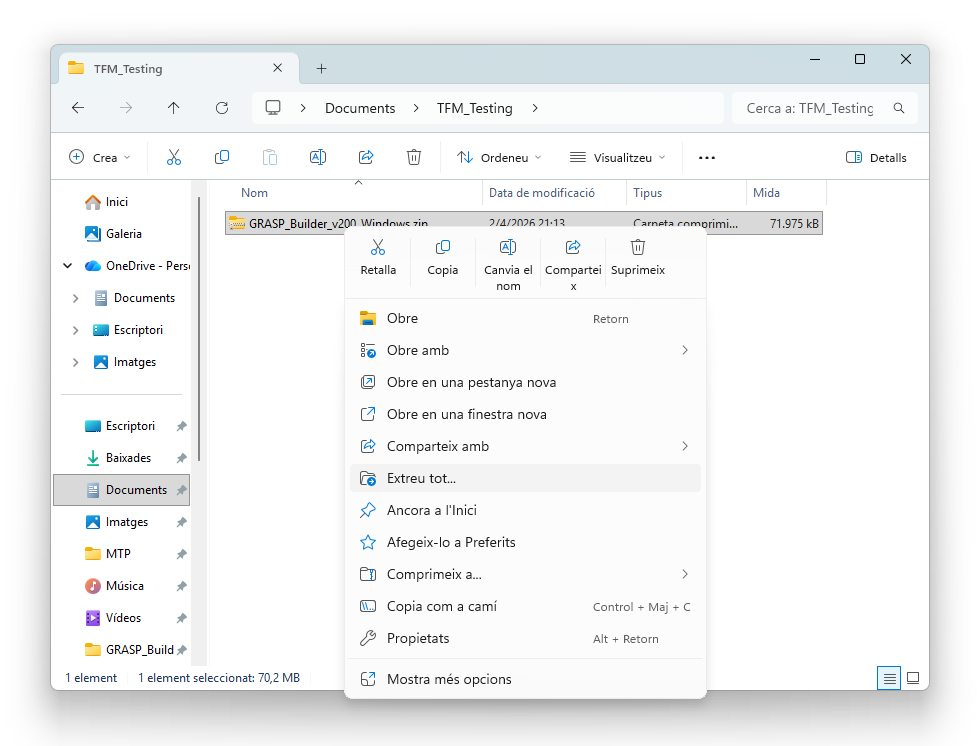
\includegraphics[width=16cm]{img/unzip.png}
\caption[Project loaded]{\footnotesize{Unzip process in Windows}}
\label{fig:UnzipWindows}
\end{figure}
{In the unzipped folder there will be an executable called GRASP\_Builder.exe and it can be executed.}
\begin{figure}[H]
\centering
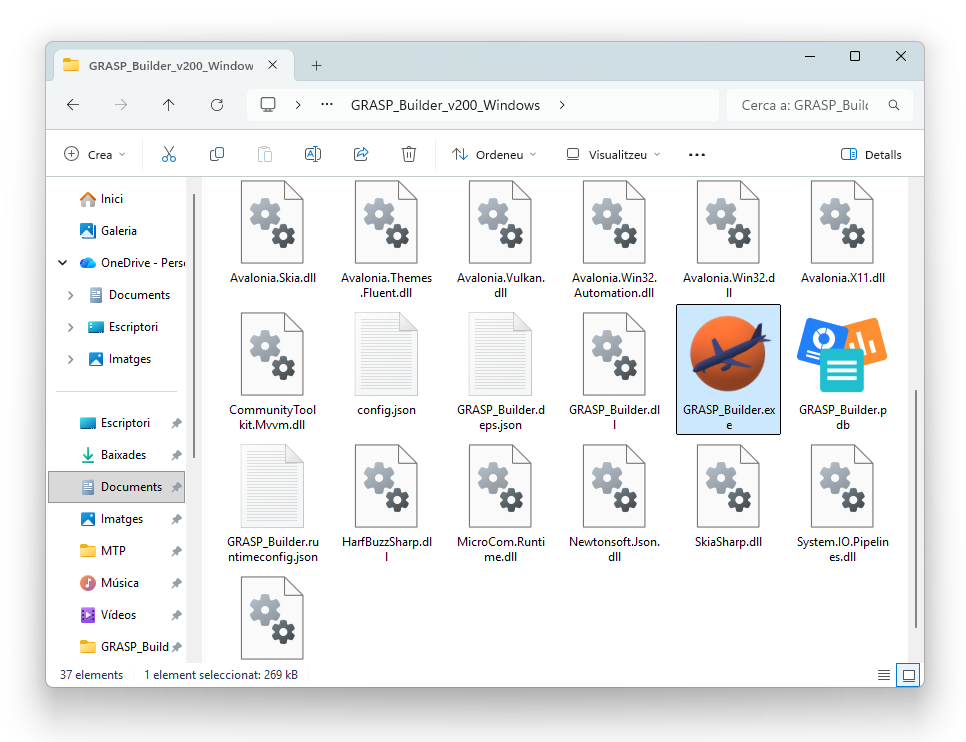
\includegraphics[width=16cm]{img/executable_windows.png}
\caption[Project loaded]{\footnotesize{Executable in Windows}}
\label{fig:ExecutableWindows}
\end{figure}
\subsection{Linux: CALCULA}
{A similar procedure needs to be followed in the Linux environment, but it can all be executed via the command line. In this case, an extra step is needed, since Linux needs an application to be specified as executable.
\smallskip\\In the desired folder, it is needed to open a command line. It can be done as it is shown in the following image:}
\begin{figure}[H]
\centering
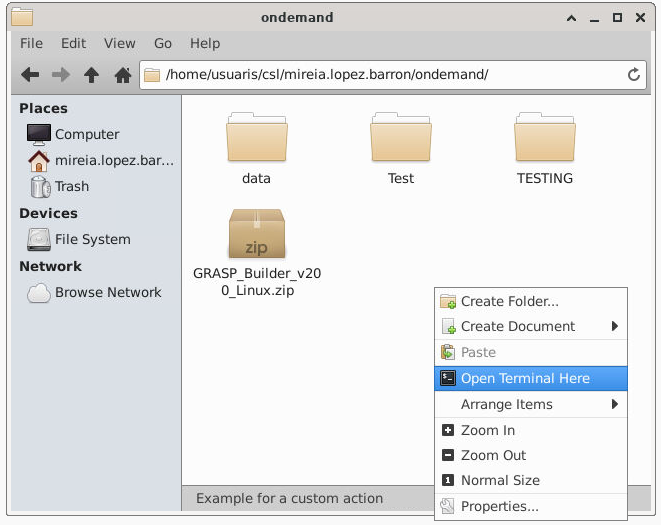
\includegraphics[width=16cm]{img/OpenCmdLinux.png}
\caption[Open cmd in Linux]{\footnotesize{Open cmd in desired folder using Linux}}
\label{fig:OpenCmdLinux}
\end{figure}
{Once it is opened, the following lines have to be executed, in order to unzip files, move to new folder and give executable permissions to the application.\smallskip}
\begin{lstlisting}
    unzip GRASP_Builder_Release_Linux.zip
    cd GRASP_Builder_Release_Linux
    chmod +x GRASP_Builder
\end{lstlisting}
{With these commands, the application has been prepared to be opened whenever it is desired by using the command:\smallskip}
\begin{lstlisting}
    ./GRASP_Builder
\end{lstlisting}
{Since this application is not shortcuted with a command, every time it is desired to be used, it has to be accessed the installation folder via command line and execute the calling command with the application name.}